\section{Teoría de grafos}
    \subsection{Conceptos básicos}
        \begin{definition}{Grafo}
            Un grafo es una terna ordenada $(V,E,\varphi)$ tal que:
            \begin{itemize}
                \item[$V$] Es un conjunto de vértices tal que $V\neq\varnothing$.
                \item[$E$] Es un conjunto de aristas tales que $E\cap V\neq\varnothing$.
                \item[$\varphi$] Es una función tal que $\varphi:E\longmapsto\{A\subset V|0\le\abs{A}\le2\}$.
            \end{itemize}
        \end{definition}
        \begin{definition}{Incidencia}
            Sea $G=(V,E,\varphi)$ un grafo. Si $v\in V$ y $e\in E$, entonces decimos que $v$ incide en $e$ y $e$ incide en $v$ si $v\in\varphi(e)$.
        \end{definition}
        \begin{definition}{Extremos de una arista}
            Sea $e\in E$, entonces a los elementos de $\varphi(e)$ los llamamos los extremos de $e$.
        \end{definition}
        \begin{definition}{Vértices adyacentes}
            Sean $u,v\in V$ decimos que $u$ y $v$ son adyacentes si $\exists\: e\in E$ tal que $\varphi(e)=\{u,v\}$.
        \end{definition}
        \begin{definition}{Aristas adyacentes}
            Sean $e,e'\in E$ decimos que $e$ y $e'$ son adyacentes si $\varphi(e)\cap\varphi(e')\neq\varnothing$.
        \end{definition}
        \begin{definition}{Bucle (Loop)}
            Sea $e\in E$, $e$ es un bucle si $\abs{\varphi(e)}=1$.
        \end{definition}
        \begin{definition}{Aristas múltiples}
            Sea $e\in E$, $e$ es una arista múltiple si $\exists\:e'\in E$ con $e\neq e'$ tal que $\varphi(e)=\varphi(e')$. De lo contrario es una arista simple.
        \end{definition}
        \begin{definition}{Grafo simple}
            Un grafo es simple si no tiene bucles ni asistas múltiples.\newline Sea $G=(V,E,\varphi)$ un grafo simple, satisface:
            $$\varphi:E\longmapsto\{A\subseteq V|\abs{A}=2\}\text{, $\varphi$ es inyectiva}$$
        \end{definition}
        \begin{definition}{Isomorfismo}
            Un isomorfismo entre las gráficas $G=(V,E,\varphi)$ y $G'=(V',E',\varphi)$
            es un par de funciones $\psi_V$ y $\psi_E$:
            \[
                \left.
                    \begin{array}{c}
                        \psi_V:V\longmapsto V' \\ 
                        \psi_E:E\longmapsto E' 
                    \end{array} 
                \right\} \text{Ambas biyectivas}
            \]
            tales que $\forall\:e\in E$, si $\varphi(e)=\{u,v\}$, entonces $\varphi(\psi_E(e))=\{\psi_V(u),\psi_V(v)\}$
        \end{definition}
    \subsection{Clases especiales de grafos}
        \begin{definition}{Grafos $K_n$}
            Sea $n\in\N$, se denota $K_n$ a los grafos simples con $n$ vértices, cualesquiera dos de ellos adyacentes.\\
            El grafo $K_n$ tiene $\binom{n}{2}$ aristas.
        \end{definition}
        
        \begin{table}[h!]
            \begin{center}
                \begin{tabular}{ccc}
                
                    \textbf{$K_1$} & \textbf{$K_2$} & \textbf{$K_3$} \\
                    % Grafo k_1
                    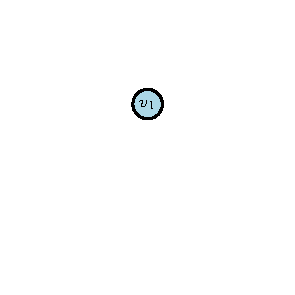
\includegraphics{Sections/Graphs/GraphsImages/GraphsKn/K1.pdf}
                    \centering 
                    &
                    % Grafo k_2
                    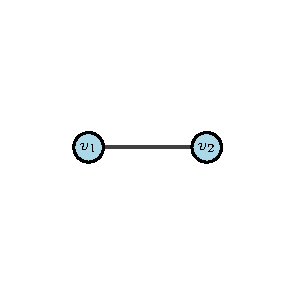
\includegraphics{Sections/Graphs/GraphsImages/GraphsKn/K2.pdf}
                    &
                    % Grafo k_3
                    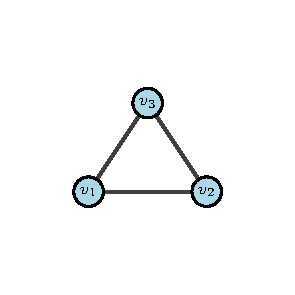
\includegraphics{Sections/Graphs/GraphsImages/GraphsKn/K3.pdf}
                    \\
                    \textbf{$K_4$} &  & \textbf{$K_5$} \\
                    % Grafo k_4
                    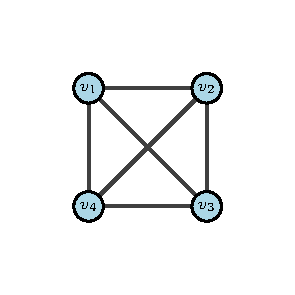
\includegraphics{Sections/Graphs/GraphsImages/GraphsKn/K4.pdf}
                    &
                    &
                    % Grafo k_5
                    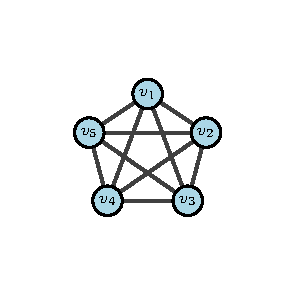
\includegraphics{Sections/Graphs/GraphsImages/GraphsKn/K5.pdf}
                \end{tabular}
              \caption{Grafos $K_n$}
              \label{tbl:grafosKn}
            \end{center}
        \end{table}

        \begin{definition}{Grafos $T_n$}
            Sea $n\in\N$ y $G=(V,E,\varphi)$ con $e_i\in E$, se denota $T_n$ a los grafos simples con $n$ vértices, con aristas de la forma:
            $$E=\{e_i|\varphi(e_i)=\{v_i,v_{i+1}\}\text{ con }1\le i\le n-1\}$$
            El grafo $T_n$ tiene $n-1$ aristas.
        \end{definition}
        \begin{table}[H]
            \begin{center}
                \begin{tabular}{ccc}
                
                    \textbf{$T_1$} & \textbf{$T_2$} & \textbf{$T_3$} \\
                    % Grafo k_1
                    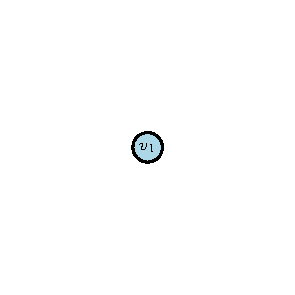
\includegraphics{Sections/Graphs/GraphsImages/GraphsTn/T1.pdf}
                    \centering 
                    &
                    % Grafo k_2
                    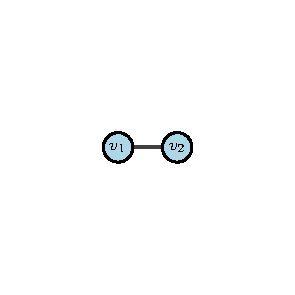
\includegraphics{Sections/Graphs/GraphsImages/GraphsTn/T2.pdf}
                    &
                    % Grafo k_3
                    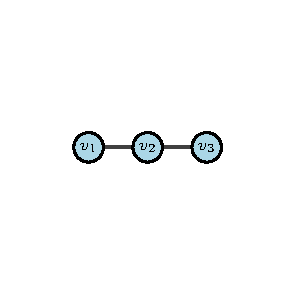
\includegraphics{Sections/Graphs/GraphsImages/GraphsTn/T3.pdf}
                    \\
                    \textbf{$T_4$} &  & \textbf{$T_5$} \\
                    % Grafo k_4
                    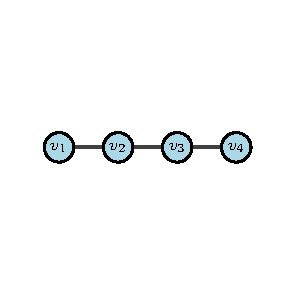
\includegraphics{Sections/Graphs/GraphsImages/GraphsTn/T4.pdf}
                    &
                    &
                    % Grafo k_5
                    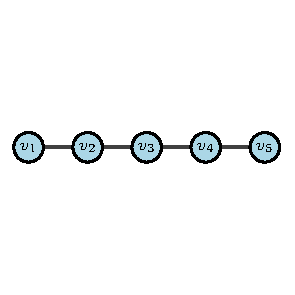
\includegraphics{Sections/Graphs/GraphsImages/GraphsTn/T5.pdf}
                \end{tabular}
              \caption{Grafos $T_n$}
              \label{tbl:grafosTn}
            \end{center}
        \end{table}
        \begin{definition}{Grafos $C_n$}
            Sea $n\in\N$ tal que $3\le n$, y $G=(V,E,\varphi)$ con $e_i\in E$, se denota $C_n$ a los grafos simples con $n$ vértices, con aristas de la forma:
            \[
                E=\left\{e_i\left|
                    \begin{array}{cl}
                        \varphi(e_i)=\{v_i,v_{i+1}\} & \text{ con }1\le i<n \\ 
                        \varphi(e_i)=\{v_i,v_1\} & \text{ con }i=n 
                    \end{array} 
                \right.\right\}
            \]
            El grafo $C_n$ tiene $n$ aristas.
        \end{definition}
        \begin{table}[H]
            \begin{center}
                \begin{tabular}{ccc}
                    \textbf{$C_3$} & \textbf{$C_4$} & \textbf{$C_5$} \\
                    % Grafo k_1
                    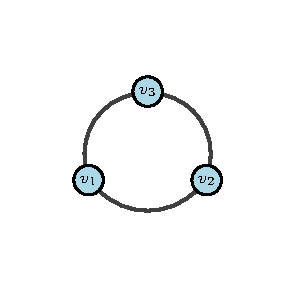
\includegraphics{Sections/Graphs/GraphsImages/GraphsCn/C3.pdf}
                    \centering 
                    &
                    % Grafo k_2
                    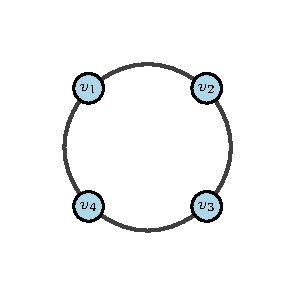
\includegraphics{Sections/Graphs/GraphsImages/GraphsCn/C4.pdf}
                    &
                    % Grafo k_3
                    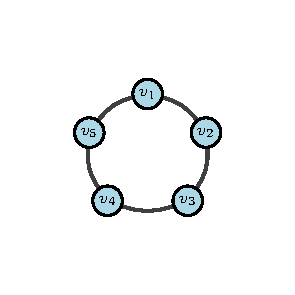
\includegraphics{Sections/Graphs/GraphsImages/GraphsCn/C5.pdf}
                \end{tabular}
              \caption{Grafos $C_n$}
              \label{tbl:grafosCn}
            \end{center}
        \end{table}
        \begin{definition}{Grafos $S_n$}
            Sea $n\in\N$ y $G=(V,E,\varphi)$ con $e_i\in E$, se denota $S_n$ a los grafos simples con $n+1$ vértices, con aristas de la forma:
            $$E=\{e_i|\varphi(e_i)=\{v_0,v_i\}\text{ con }1\le i\le n\}$$
            El grafo $S_n$ tiene $n$ aristas.
        \end{definition}
        \begin{table}[H]
            \begin{center}
                \begin{tabular}{ccc}
                
                    \textbf{$S_1$} & \textbf{$S_2$} & \textbf{$S_3$} \\
                    % Grafo k_1
                    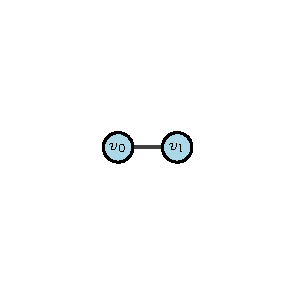
\includegraphics{Sections/Graphs/GraphsImages/GraphsSn/S1.pdf}
                    \centering 
                    &
                    % Grafo k_2
                    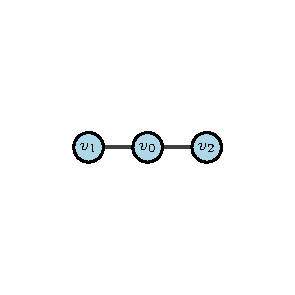
\includegraphics{Sections/Graphs/GraphsImages/GraphsSn/S2.pdf}
                    &
                    % Grafo k_3
                    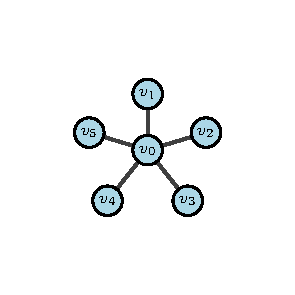
\includegraphics{Sections/Graphs/GraphsImages/GraphsSn/S5.pdf}
                    \\
                    \textbf{$S_4$} &  & \textbf{$S_5$} \\
                    % Grafo k_4
                    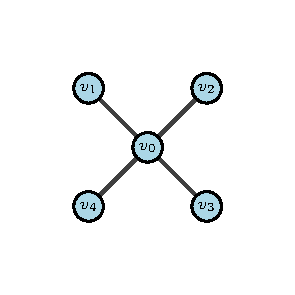
\includegraphics{Sections/Graphs/GraphsImages/GraphsSn/S4.pdf}
                    &
                    &
                    % Grafo k_5
                    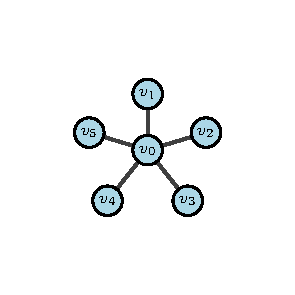
\includegraphics{Sections/Graphs/GraphsImages/GraphsSn/S5.pdf}
                \end{tabular}
              \caption{Grafos $S_n$}
              \label{tbl:grafosTn}
            \end{center}
        \end{table}
        \begin{definition}{Grafos $W_n$}
            Sea $n\in\N$ y $G=(V,E,\varphi)$ con $e_i\in E$, se denota $W_n$ a los grafos simples con $n+1$ vértices, con aristas de la forma:
            \[
                E=\{e_i|\varphi(e_i)=\{v_0,v_i\}\text{ con }1\le i\le n\}\cup
                \left\{e_i\left|
                    \begin{array}{cl}
                        \varphi(e_i)=\{v_i,v_{i+1}\} & \text{ con }1\le i<n \\ 
                        \varphi(e_i)=\{v_i,v_1\} & \text{ con }i=n 
                    \end{array} 
                \right.\right\}
            \]
            El grafo $W_n$ tiene $2n$ aristas.
        \end{definition}
        \begin{table}[H]
            \begin{center}
                \begin{tabular}{cc}
                
                    \textbf{$W_2$} & \textbf{$W_3$}\\
                    % Grafo k_1
                    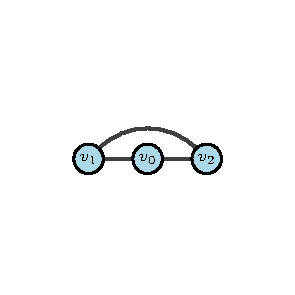
\includegraphics{Sections/Graphs/GraphsImages/GraphsWn/W2.pdf}
                    \centering 
                    &
                    % Grafo k_2
                    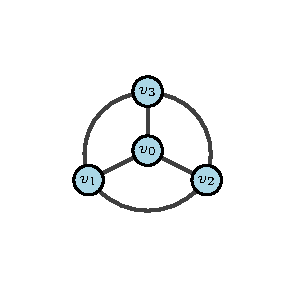
\includegraphics{Sections/Graphs/GraphsImages/GraphsWn/W3.pdf}
                    \\
                    \textbf{$W_4$} & \textbf{$W_5$} \\
                    % Grafo k_4
                    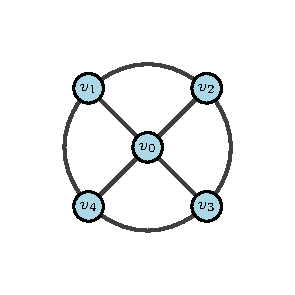
\includegraphics{Sections/Graphs/GraphsImages/GraphsWn/W4.pdf}
                    &
                    % Grafo k_5
                    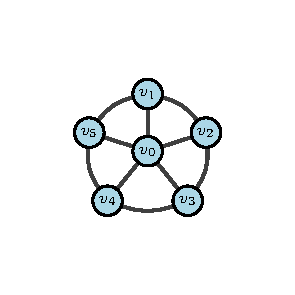
\includegraphics{Sections/Graphs/GraphsImages/GraphsWn/W5.pdf}
                \end{tabular}
              \caption{Grafos $W_n$}
              \label{tbl:grafosTn}
            \end{center}
        \end{table}